\documentclass[12pt]{article}
\usepackage[top=2.8cm,bottom=2.8cm,left=2.5cm,right=2.5cm]{geometry}
\usepackage[utf8]{inputenc}
\usepackage[T1]{fontenc}
\usepackage{amsmath,amssymb}
\usepackage{booktabs}
\usepackage{graphicx}
\usepackage{enumitem}
\usepackage{setspace}
\usepackage{parskip}
\usepackage{tikz}
\usepackage{pgfplots}
\pgfplotsset{compat=1.18}
\usepackage{fancyhdr}
\setlength{\headheight}{14pt}
\usepackage{xcolor}
\usepackage{mdframed}
\usepackage{tcolorbox}
\tcbuselibrary{breakable,skins}

\pagestyle{fancy}
\fancyhf{}
\fancyhead[L]{\small ECON 311 --- Fall 2026}
\fancyhead[R]{\small Solutions -- Practice Problem Set 1}
\fancyfoot[C]{\small \thepage}
\renewcommand{\headrulewidth}{0.4pt}

\setlength{\parskip}{6pt}
\onehalfspacing

% Solution box style
\newenvironment{soln}{%
  \begin{tcolorbox}[
    breakable,
    colback=blue!4!white,
    colframe=blue!50!black,
    title={\textbf{Solution}},
    fonttitle=\small,
    left=4pt, right=4pt, top=4pt, bottom=4pt
  ]
}{%
  \end{tcolorbox}
}

\begin{document}

%-----------------------------------------------------------------------
% Title block
%-----------------------------------------------------------------------
\begin{center}
{\LARGE \textbf{Solutions -- Practice Problem Set 1}}\\[10pt]
  {\large \textbf{ECON 311 --- Intermediate Macroeconomics --- Fall 2026}}\\[6pt]

\end{center}

\bigskip\hrule\bigskip

%-----------------------------------------------------------------------


%-----------------------------------------------------------------------
\noindent\textbf{Problem 1} \quad Growth-rate arithmetic.

\bigskip
\textit{Background:} The key rule is that if $z = u^a v^b$, then
$g_z = a\,g_u + b\,g_v$, where growth rates of products add and growth
rates of ratios subtract.

\begin{soln}
\begin{enumerate}[label=(\alph*),leftmargin=2em,itemsep=6pt]
  \item $z = x^2 y^3$ \\
        $\Rightarrow g_z = 2g_x + 3g_y$

  \item $z = \dfrac{x^{0.6}}{y^{0.4}} = x^{0.6}\,y^{-0.4}$ \\
        $\Rightarrow g_z = 0.6\,g_x - 0.4\,g_y$

  \item $z = x^{-0.5}\left(\dfrac{1}{w}\right)^{0.3}y^{0.8}
             = x^{-0.5}\,w^{-0.3}\,y^{0.8}$ \\
        $\Rightarrow g_z = -0.5\,g_x - 0.3\,g_w + 0.8\,g_y$

  \item $z = \left(\dfrac{xy}{w^2}\right)^{1/2} = x^{1/2}\,y^{1/2}\,w^{-1}$ \\
        $\Rightarrow g_z = \tfrac{1}{2}g_x + \tfrac{1}{2}g_y - g_w$
\end{enumerate}
\end{soln}

\bigskip

%-----------------------------------------------------------------------
\noindent\textbf{Problem 2} \quad Returns to scale.

\bigskip
\textit{Method:} Scale both inputs by $\gamma > 0$:
replace $K \to \gamma K$ and $L \to \gamma L$.
If $F(\gamma K, \gamma L) = \gamma^\lambda F(K,L)$, the function has:
$\lambda>1$ (IRS), $\lambda=1$ (CRS), $\lambda<1$ (DRS).
For a Cobb--Douglas $Y = AK^\alpha L^\beta$: check $\alpha+\beta$.

\begin{soln}
\begin{enumerate}[label=(\alph*),leftmargin=2em,itemsep=8pt]
  \item $Y = \bar{A}K^{1/4}L^{3/4}$: exponents sum to $\tfrac{1}{4}+\tfrac{3}{4}=1$.
        \textbf{Constant returns to scale (CRS).}

  \item $Y = K^{0.6}L^{0.6}$: exponents sum to $0.6+0.6=1.2>1$.
        \textbf{Increasing returns to scale (IRS).}

  \item $Y = K^{1/3}L^{2/3} + \bar{A}$: the exponents of the Cobb--Douglas part
        sum to 1, but there is an additive constant, so we cannot read off RTS
        from the exponents alone.  Apply the definition:
        \[
          F(\gamma K,\gamma L)
          = (\gamma K)^{1/3}(\gamma L)^{2/3} + \bar{A}
          = \gamma K^{1/3}L^{2/3} + \bar{A}.
        \]
        Compare with $\gamma F(K,L) = \gamma K^{1/3}L^{2/3} + \gamma\bar{A}$.
        The difference is
        \[
          F(\gamma K,\gamma L) - \gamma F(K,L)
          = \bar{A} - \gamma\bar{A} = (1-\gamma)\bar{A}.
        \]
        For $\gamma > 1$, this is negative, meaning $F(\gamma K,\gamma L) < \gamma F(K,L)$.
        \textbf{Decreasing returns to scale (DRS).}

        \textit{Economic interpretation:} The constant $\bar{A}$ (e.g., a fixed
        factor such as land or a licence) is not scaled, so doubling inputs
        produces less than double the output.

  \item $Y = K + K^{0.5}L^{0.5}$: apply the definition.
        \[
          F(\gamma K,\gamma L)
          = \gamma K + (\gamma K)^{0.5}(\gamma L)^{0.5}
          = \gamma K + \gamma K^{0.5}L^{0.5}
          = \gamma\bigl(K + K^{0.5}L^{0.5}\bigr)
          = \gamma F(K,L).
        \]
        \textbf{Constant returns to scale (CRS).}
\end{enumerate}
\end{soln}

\bigskip

%-----------------------------------------------------------------------
\noindent\textbf{Problem 3} \quad National income accounting.

\bigskip
\textit{Setup summary:}
\begin{itemize}[leftmargin=1.5em,itemsep=2pt]
  \item Lumber company: pays \$18{,}000 wages; sells 400\,m$^3$ to furniture
        mfr.\ at \$60/m$^3$ $= \$24{,}000$; sells planks to households for
        \$9{,}000.
  \item Furniture manufacturer: buys timber \$24{,}000; pays wages \$30{,}000;
        makes 50 chairs.  Sales: 35 to households $\times \$1{,}200=\$42{,}000$;
        10 to government $\times \$1{,}200=\$12{,}000$;
        5 exported $\times \$1{,}400=\$7{,}000$.
        Total revenue $= \$61{,}000$.
\end{itemize}

\begin{soln}
\textbf{(a) Expenditure approach}

Count only \emph{final} goods (those not used as intermediate inputs):
\begin{align*}
  C &= \text{planks to households} + \text{chairs to households}
       = 9{,}000 + 42{,}000 = \$51{,}000 \\
  G &= \text{chairs to government} = \$12{,}000 \\
  NX &= \text{exported chairs} = \$7{,}000 \\
  I &= 0 \quad \text{(no capital investment described)}
\end{align*}
\[
  \boxed{GDP = C + G + NX = 51{,}000 + 12{,}000 + 7{,}000 = \$70{,}000}
\]

\textbf{(b) Income approach}

\textit{Labour income:}
\[
  18{,}000 + 30{,}000 = \$48{,}000
\]

\textit{Capital income (profit) --- each firm:}

Lumber company revenue $= 24{,}000 + 9{,}000 = \$33{,}000$.
No intermediate inputs.
Profit $= 33{,}000 - 18{,}000 = \$15{,}000$.

Furniture manufacturer revenue $= 42{,}000 + 12{,}000 + 7{,}000 = \$61{,}000$.
Costs: labour \$30{,}000 + timber \$24{,}000 $= \$54{,}000$.
Profit $= 61{,}000 - 54{,}000 = \$7{,}000$.

\[
  GDP = 48{,}000 + 15{,}000 + 7{,}000 = \boxed{\$70{,}000}
\]

\textbf{(c) Value-added approach}

Value added equals revenue minus the cost of intermediate inputs.

\medskip
\begin{tabular}{lrr}
  \toprule
  Firm & Revenue & Intermediate inputs \\
  \midrule
  Lumber company & \$33{,}000 & \$0 \\
  Furniture manufacturer & \$61{,}000 & \$24{,}000 \\
  \midrule
  \multicolumn{3}{l}{Value added: lumber $= \$33{,}000$; furniture $= \$37{,}000$} \\
  \bottomrule
\end{tabular}

\[
  GDP = 33{,}000 + 37{,}000 = \boxed{\$70{,}000}
\]

\textbf{(d)} All three methods yield \$70{,}000. \checkmark
\end{soln}

\bigskip
\newpage

%-----------------------------------------------------------------------


%-----------------------------------------------------------------------
\noindent\textbf{Problem 4} \quad Real GDP, nominal GDP, and the GDP deflator.

\begin{soln}
\textbf{(a) Nominal GDP in Year 2}

Final goods only, at Year-2 prices:
\begin{align*}
  C &= \text{planks to households} + \text{chairs to households}
       = 11{,}500 + 35 \times 1{,}500 = 11{,}500 + 52{,}500 = \$64{,}000 \\
  G &= 10 \times 1{,}500 = \$15{,}000 \\
  NX &= 5 \times 1{,}700 = \$8{,}500
\end{align*}
\[
  \text{Nominal GDP}_2 = 64{,}000 + 15{,}000 + 8{,}500 = \boxed{\$87{,}500}
\]

\textbf{(b) Real GDP in Year 2 (Year-1 base prices)}

Quantities are identical to Year 1; prices are Year-1 prices:
\[
  \text{Real GDP}_2 = \text{GDP}_1 = \$70{,}000
\]
Real GDP growth rate $= \dfrac{70{,}000 - 70{,}000}{70{,}000} = \mathbf{0\%}$.

\textbf{(c) GDP deflator for Year 2}

\[
  \text{GDP Deflator}_2 = \frac{\text{Nominal GDP}_2}{\text{Real GDP}_2}
  = \frac{87{,}500}{70{,}000} \approx 1.250
\]
Percentage change in the price level $= (1.250 - 1.000) \times 100\% = \mathbf{25\%}$.

\textbf{(d) Economic interpretation}

Real GDP measures the value of output at constant (base-year) prices, so it
captures only changes in the \emph{quantity} of goods produced.  Since all
quantities remained the same in Year 2, real GDP did not change.  Nominal GDP
rose solely because prices rose.  The GDP deflator isolates this pure price
change: the general price level rose by 25\% between Year 1 and Year 2.
\end{soln}

\bigskip
\newpage
%-----------------------------------------------------------------------
\noindent\textbf{Problem 5} \quad Economic convergence.

\begin{soln}
\textbf{(a) Catch-up formula}

Set $Y^A_t = Y^B_t$:
\[
  5{,}000\,(1.04)^{t^*} = 24{,}000\,(1.02)^{t^*}
\]
\[
  \left(\frac{1.04}{1.02}\right)^{t^*} = \frac{24{,}000}{5{,}000} = 4.8
\]
\[
  t^* \cdot \ln\!\left(\frac{1.04}{1.02}\right) = \ln(4.8)
  \quad\Rightarrow\quad
  t^* = \frac{\ln(4.8)}{\ln(1.04/1.02)}
  = \frac{1.5686}{0.019608} \approx \mathbf{80.8\ \text{years}}
\]
Country Alder catches up approximately in the year $2000 + 81 = \mathbf{2081}$.

\textbf{(b) Accelerated early growth}

For the first 15 years Alder grows at 7\%; thereafter at 4\%.
Country Birch grows at 2\% throughout.  Set them equal at time $T$
(years after 2000, where $T > 15$):
\[
  5{,}000\,(1.07)^{15}\,(1.04)^{T-15}
  = 24{,}000\,(1.02)^{T}
\]
\[
  \frac{(1.04)^T}{(1.04)^{15}\,(1.02)^T}
  = \frac{24{,}000}{5{,}000\,(1.07)^{15}}
\]
\[
  \left(\frac{1.04}{1.02}\right)^T
  = \frac{24{,}000}{5{,}000\,(1.07)^{15}}\,(1.04)^{15}
\]

Calculate the numerical constants:
$(1.07)^{15} \approx 2.7590$, $(1.04)^{15} \approx 1.8009$.

\[
  \left(\frac{1.04}{1.02}\right)^T
  = \frac{24{,}000}{5{,}000 \times 2.7590} \times 1.8009
  = \frac{24{,}000 \times 1.8009}{13{,}795}
  \approx \frac{43{,}222}{13{,}795}
  \approx 3.1330
\]
\[
  T = \frac{\ln(3.1332)}{\ln(1.04/1.02)}
  = \frac{1.1422}{0.019608}
  \approx \mathbf{58.3\ \text{years}}
\]

With the 7\% early growth, Alder catches up approximately in year
$2000 + 58 = \mathbf{2058}$ --- about 23 years sooner.

\textbf{(c) Economic interpretation}

The accelerated early growth compresses the initial income gap much faster,
so Alder needs fewer years at the moderate 4\% rate to close the remaining
gap.  In practice, a country could achieve 7\% growth through institutional
reforms, technology transfer, foreign direct investment, or capital
accumulation from a very low capital base (consistent with the Solow model:
a poor country far below its steady state has a high marginal product of
capital and thus high growth rates).
\end{soln}

\bigskip

%-----------------------------------------------------------------------
\noindent\textbf{Problem 6} \quad From aggregate to per-capita variables.

\begin{soln}
\textbf{(a)} Divide both sides of $Y_t = AK_t^\alpha L_t^{1-\alpha}$
by $L_t$:
\[
  \frac{Y_t}{L_t}
  = A\,\frac{K_t^\alpha L_t^{1-\alpha}}{L_t}
  = A\,\frac{K_t^\alpha}{L_t^\alpha}
  = A\left(\frac{K_t}{L_t}\right)^\alpha
  = A k_t^\alpha.
\]
Therefore $y_t = Ak_t^\alpha$. \hfill $\square$

\textbf{(b)} Start from the capital accumulation equation and substitute
$I_t = \bar{s}Y_t$:
\[
  K_{t+1} = (1-\delta)K_t + \bar{s}Y_t.
\]
Subtract $K_t$ from both sides:
\[
  \Delta K_{t+1} = \bar{s}Y_t - \delta K_t.
\]
Divide both sides by $L_t$:
\[
  \frac{\Delta K_{t+1}}{L_t} = \bar{s}\,\frac{Y_t}{L_t} - \delta\,\frac{K_t}{L_t}
  = \bar{s}\,y_t - \delta\,k_t. \tag{$*$}
\]

Now use the approximation for growth rates.  Since $k_t = K_t/L_t$:
\[
  g_k \approx g_K - g_L = \frac{\Delta K_{t+1}}{K_t} - \bar{n}.
\]
Multiplying both sides by $k_t$:
\[
  \frac{\Delta k_{t+1}}{1} = k_t \cdot g_k
  = \frac{\Delta K_{t+1}}{K_t}\cdot k_t - \bar{n}\,k_t
  = \frac{\Delta K_{t+1}}{L_t} - \bar{n}\,k_t. \tag{$**$}
\]
Substituting $(*)$ into $(**)$:
\[
  \Delta k_{t+1} = \bar{s}\,y_t - \delta k_t - \bar{n}\,k_t
  = \bar{s}\,y_t - (\delta + \bar{n})\,k_t. \hfill \square
\]

\textbf{(c) Economic interpretation}

\begin{itemize}[leftmargin=1.5em,itemsep=4pt]
  \item $\bar{s}\,y_t$: \textbf{actual investment per person.}
        This is the amount of new capital being added to the economy
        per worker each period.

  \item $\delta\,k_t$: \textbf{depreciation.}  A fraction $\delta$ of the
        existing capital stock per worker wears out each period.

  \item $\bar{n}\,k_t$: \textbf{capital dilution.}  Even if no capital
        depreciates, a growing population spreads the existing capital across
        more workers, reducing capital per person.

  \item The sum $(\delta+\bar{n})k_t$ is the \textbf{break-even investment}:
        the investment needed just to keep $k$ constant.

  \item $\Delta k_{t+1} > 0$ when actual investment exceeds break-even
        investment; capital per worker rises.  At steady state,
        $\bar{s}\,y^* = (\delta+\bar{n})k^*$.
\end{itemize}
\end{soln}

\bigskip

%-----------------------------------------------------------------------

%-----------------------------------------------------------------------
\noindent\textbf{Problem 7} \quad Solow model: steady state.

\begin{soln}
\textbf{(a) Steady-state derivation} ($\alpha = 1/3$)

At steady state $\Delta k_{t+1} = 0$:
\[
  \bar{s}\,y^* = (\delta+\bar{n})\,k^*.
\]
Substitute $y^* = A k^{*1/3}$:
\[
  \bar{s}\,A\,k^{*1/3} = (\delta+\bar{n})\,k^*.
\]
Divide both sides by $k^{*1/3}$:
\[
  \bar{s}\,A = (\delta+\bar{n})\,k^{*2/3}
  \quad\Rightarrow\quad
  k^{*2/3} = \frac{\bar{s}A}{\delta+\bar{n}}
  \quad\Rightarrow\quad
  \boxed{k^* = \left(\frac{\bar{s}A}{\delta+\bar{n}}\right)^{3/2}}
\]
Then:
\[
  y^* = A k^{*1/3}
  = A \left(\frac{\bar{s}A}{\delta+\bar{n}}\right)^{1/2}
  = \boxed{A^{3/2}\left(\frac{\bar{s}}{\delta+\bar{n}}\right)^{1/2}}
\]

\textbf{(b) Effect of an increase in $\bar{s}$}

Both $k^*$ and $y^*$ are increasing functions of $\bar{s}$ (the exponents
are positive).  A higher savings rate means more investment per worker each
period, so the break-even condition is satisfied at a higher level of capital
and output per worker.

\textit{Economic interpretation:} When households save more, a larger share
of output is channelled into investment.  This raises the capital stock per
worker and, through the production function, raises output per worker in the
long run.

\textbf{(c) Effect of an increase in $\bar{n}$}

$(\delta+\bar{n})$ appears in the denominator (with a positive exponent),
so both $k^*$ and $y^*$ \emph{decrease} when $\bar{n}$ rises.

\textit{Economic interpretation:} Faster population growth means each unit of
new investment must be spread over more workers just to maintain capital per
worker (the dilution effect is larger).  This leaves less net investment for
deepening capital, pushing the steady-state capital-labour ratio down.
\end{soln}

\bigskip

%-----------------------------------------------------------------------
\noindent\textbf{Problem 8} \quad Solow model: numerical dynamics.

\begin{soln}
\textbf{(a) Steady-state values}

Parameters: $A=1,\ \bar{s}=0.25,\ \delta=0.06,\ \bar{n}=0.02$,
so $\delta+\bar{n}=0.08$.

\[
  k^* = \left(\frac{0.25\times 1}{0.08}\right)^{3/2}
  = (3.125)^{3/2}
  = 3.125 \times \sqrt{3.125}
  \approx 3.125 \times 1.7678
  \approx \mathbf{5.523}
\]
\[
  y^* = 1^{3/2}\left(\frac{0.25}{0.08}\right)^{1/2}
  = (3.125)^{1/2}
  \approx \mathbf{1.768}
\]

\textbf{(b) Capital dynamics} starting from $k_1 = 6$

The accumulation equation is:
$\Delta k_{t+1} = 0.25\,k_t^{1/3} - 0.08\,k_t.$

\medskip
\textit{Period 1 $\to$ 2}:
\[
  y_1 = 6^{1/3} \approx 1.8171, \quad
  \Delta k_2 = 0.25(1.8171) - 0.08(6)
  = 0.4543 - 0.4800 = -0.0257
\]
$k_2 = 6 - 0.0257 = 5.9743$.

\textit{Period 2 $\to$ 3}:
\[
  y_2 = 5.9743^{1/3} \approx 1.8149, \quad
  \Delta k_3 = 0.25(1.8149) - 0.08(5.9743)
  = 0.4537 - 0.4779 = -0.0242
\]
$k_3 \approx 5.9501$.

\textit{Period 3 $\to$ 4}: $k_3 \approx 5.9501$
\[
  y_3 \approx 5.9501^{1/3} \approx 1.8128, \quad
  \Delta k_4 \approx 0.25(1.8128) - 0.08(5.9501)
  = 0.4532 - 0.4760 = -0.0228
\]

\textit{Period 4 $\to$ 5}: $k_4 \approx 5.9273$
\[
  y_4 \approx 5.9273^{1/3} \approx 1.8108, \quad
  \Delta k_5 \approx 0.25(1.8108) - 0.08(5.9273)
  = 0.4527 - 0.4742 = -0.0215
\]

Summary:
\[
  \Delta k_2 \approx -0.026,\quad
  \Delta k_3 \approx -0.024,\quad
  \Delta k_4 \approx -0.023,\quad
  \Delta k_5 \approx -0.022
\]

\textbf{(c) Pattern and explanation}

The changes $\Delta k_t$ are \emph{negative} but \emph{decreasing in
absolute value}---capital per worker is falling, but more and more slowly.
This occurs because $k_1 = 6 > k^* \approx 5.52$: the economy starts
\emph{above} its steady state.  The break-even investment exceeds actual
investment, so $k$ falls each period.  As $k$ approaches $k^*$, the gap
between actual and break-even investment shrinks, slowing the rate of
decline.

\textbf{(d) Above or below steady state?}

$k_1 = 6 > k^* \approx 5.52$, so the economy is \textbf{above} its steady
state.  This is confirmed by $\Delta k_2 < 0$: capital per worker is
declining toward $k^*$.
\end{soln}

\bigskip

%-----------------------------------------------------------------------
\noindent\textbf{Problem 9} \quad Solow diagram.

\begin{soln}
The two curves in the Solow diagram are:
\begin{itemize}[leftmargin=1.5em,itemsep=3pt]
  \item \textbf{Actual investment per worker}: $\bar{s}\,f(k) = 0.25\,k^{1/3}$
        (concave, passes through the origin).
  \item \textbf{Break-even investment}: $(\delta+\bar{n})\,k = 0.08\,k$
        (linear through the origin, slope $= 0.08$).
\end{itemize}

The steady state $k^*$ is where the two curves intersect:
$0.25\,k^{*1/3} = 0.08\,k^*$, giving $k^* \approx 5.52$.

\bigskip
\begin{center}
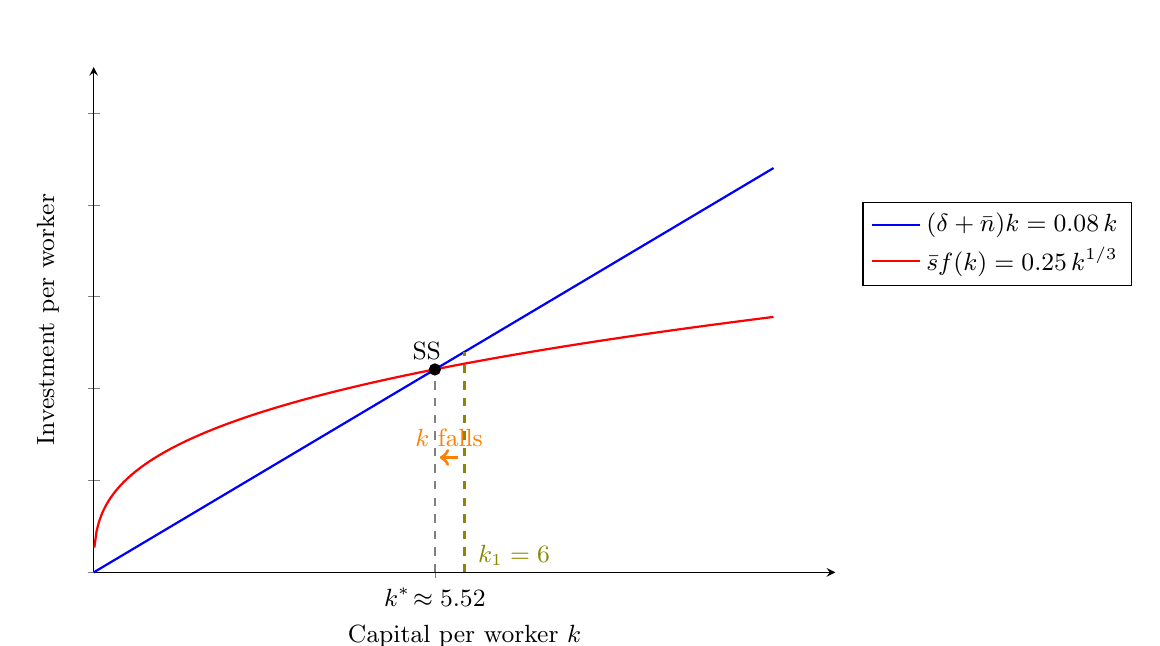
\begin{tikzpicture}
  \begin{axis}[
    width=11cm, height=8cm,
    xmin=0, xmax=12,
    ymin=0, ymax=1.1,
    xlabel={Capital per worker $k$},
    ylabel={Investment per worker},
    xtick={5.52},
    xticklabels={$k^*\!\approx 5.52$},
    ytick={},
    yticklabels={},
    axis lines=left,
    clip=false,
    legend style={at={(1.4,.65)},anchor=east},
    every axis label/.style={font=\small},
    tick label style={font=\small},
  ]
  % Break-even investment: 0.08*k
  \addplot[blue, thick, domain=0:11, samples=200]
    {0.08*x};
  \addlegendentry{\small$(\delta+\bar{n})k = 0.08\,k$}

  % Actual investment: 0.25*k^(1/3)
  \addplot[red, thick, domain=0.01:11, samples=300]
    {0.25*x^(1/3)};
  \addlegendentry{\small$\bar{s}f(k) = 0.25\,k^{1/3}$}

  % Steady state k*
  \addplot[dashed, gray, thick] coordinates {(5.52,0)(5.52,0.4416)};
  \node[below] at (axis cs:5.52,0) {};

  % Initial k_1 = 6
  \addplot[dashed, olive, thick] coordinates {(6,0)(6,0.48)};
  \node[below, olive] at (axis cs:6.8,0.08) {\small $k_1=6$};

  % Arrow showing direction of movement (from k1 toward k*)
  \draw[->, very thick, orange]
    (axis cs:5.9,0.25) -- (axis cs:5.6,0.25)
    node[midway,above,font=\small,orange] {$k$ falls};

  % Steady-state dot
  \filldraw[black] (axis cs:5.52,0.4416) circle (2pt);
  \node[above right, font=\small] at (axis cs:5,0.4416) {SS};

  \end{axis}
\end{tikzpicture}
\end{center}

\textbf{(a)} The concave curve is actual investment $\bar{s}f(k)$; the
straight line is break-even investment $(\delta+\bar{n})k$.  They cross at
$k^* \approx 5.52$ (labelled ``SS'').

\textbf{(b)} The initial position $k_1 = 6$ is marked to the right of $k^*$.

\textbf{(c)} Since $k_1 > k^*$, break-even investment exceeds actual
investment at $k_1$.  The orange arrow shows $k$ moving left (decreasing)
toward $k^*$.

\textbf{(d) Effect of an increase in $\delta$}

A higher depreciation rate raises the slope of the break-even investment
line $(\delta+\bar{n})k$.  The actual investment curve $\bar{s}f(k)$ does
not change.  The two curves now intersect at a lower value of $k$, so
$k^*$ falls.  Economically, more capital is lost to depreciation each period,
reducing the steady-state capital per worker.
\end{soln}

\bigskip

%-----------------------------------------------------------------------


%-----------------------------------------------------------------------
\noindent\textbf{Problem 10} \quad Comparative statics and policy analysis.

\begin{soln}
\textbf{(a) Transitional dynamics after a savings-rate increase}

At the old steady state $k^*$, actual investment equals break-even investment:
$\bar{s}y^* = (\delta+\bar{n})k^*$.  When $\bar{s}$ rises to $\bar{s}'$,
actual investment immediately becomes $\bar{s}'y^* > (\delta+\bar{n})k^*$,
so $\Delta k_{t+1} > 0$: capital per worker begins to rise.

As $k$ rises, $y = Ak^\alpha$ also rises (but at a decreasing marginal rate
because $\alpha < 1$), while break-even investment $(\delta+\bar{n})k$ rises
linearly.  The gap between actual and break-even investment therefore narrows,
and the growth of $k$ slows down.  The process continues until a new, higher
steady state ${k^*}'$ is reached, at which point $\bar{s}'y^{*\prime} =
(\delta+\bar{n})k^{*\prime}$ and $\Delta k_{t+1} = 0$ again.

\textbf{(b) Algebraic proof that higher $\bar{s}$ implies higher $y^*$}

From Problem 7(a):
\[
  y^* = A^{3/2}\left(\frac{\bar{s}}{\delta+\bar{n}}\right)^{1/2}.
\]
Taking the partial derivative with respect to $\bar{s}$:
\[
  \frac{\partial y^*}{\partial \bar{s}}
  = A^{3/2} \cdot \tfrac{1}{2}\left(\frac{\bar{s}}{\delta+\bar{n}}\right)^{-1/2}
    \cdot \frac{1}{\delta+\bar{n}} > 0.
\]
Since $A$, $\bar{s}$, $\delta$, $\bar{n}$ are all positive, this derivative
is strictly positive.  Therefore a higher $\bar{s}$ implies a higher $y^*$,
all else equal. \hfill $\square$

\textbf{(c) Conditional vs.\ absolute convergence}

\textit{Absolute convergence} would predict that all countries grow faster
the poorer they are, unconditionally, and that all countries converge to the
same income level in the long run.

The Solow model predicts \textit{conditional convergence}: a country converges
to its own steady state $y^*$.  Because $y^*$ depends on country-specific
parameters ($\bar{s},\delta,\bar{n},A$), two countries with the same
\emph{current} income may be going in very different directions.  A poor
country converges to a high $y^*$ if it has a high savings rate; a rich
country with a low savings rate might converge to a lower $y^*$.

Conditional convergence is consistent with the empirical finding that
countries converge when one controls for savings rates, population growth,
and other structural parameters---but not unconditionally.

\textbf{(d) Long-run growth and the need for technological progress}

At the steady state of the basic Solow model, $\Delta k_{t+1} = 0$ and
therefore $\Delta y_{t+1} = 0$.  Output per capita is constant in the long
run; the growth rate of output per capita is zero.

This is in tension with the experience of developed economies, which have
sustained positive per-capita growth for over a century.  The basic model
implies that, without technological progress, capital accumulation alone
cannot sustain long-run growth (diminishing returns to capital ensure that
the marginal product eventually falls to the break-even level).

\textit{Extension:} The standard resolution is to introduce \textbf{labour-augmenting
technological progress} at rate $\bar{g}$: $Y_t = K_t^\alpha (A_t L_t)^{1-\alpha}$
with $A_t = A_0(1+\bar{g})^t$.  The model then has a balanced growth path
along which output per \emph{effective} worker is constant, but output per
\emph{actual} worker grows at rate $\bar{g}$---matching the long-run
experience of developed economies.
\end{soln}



\end{document}
